\documentclass{beamer}
\usetheme{Berkeley}
\title{Matrix Project}
\subtitle{EE1390: Intro to AI and ML}
\author{Tejas Meshram\inst{1} \and Abhishek K. Singh\inst{2}}
\institute[IIT Hyderabad]
{
  \inst{1}%
  ME17BTECH11046
  \and
  \inst{2}%
  EP17BTECH11020
}
\date{\today}
\subject{Analysis}
\AtBeginSubsection[]
{
  \begin{frame}<beamer>{Analysis}
    \tableofcontents[currentsection,currentsubsection]
  \end{frame}
}

\begin{document}

\begin{frame}
  \titlepage
\end{frame}

\begin{frame}{Problem Solving Strategy}
  \tableofcontents
\end{frame}

\section{Theoretical Computation}

\subsection{}

\begin{frame}{Matrix problem in coordinate geometry}{From JEE Main 2018}
  \begin{itemize}
\item If $\textbf{\beta}$ is one of the angles between the normals of the ellipse $\textbf{X}^TV\textbf{X} = 9$ at
the points
$\begin{bmatrix}
           3 \cos\theta\\
           \sqrt{3}\sin\theta \\
  \end{bmatrix}$
  ,
$\begin{bmatrix}
           -3 \sin\theta \\
           \sqrt{3}\cos\theta \\
  \end{bmatrix}$
  ; $\theta \epsilon (0, \frac{\pi}{2})$, 
  $V = \begin{bmatrix}
           1 & 0 \\
           0 & 3 \\
  \end{bmatrix}$
  ; then $\frac{2\cot\textbf{$\beta$}}{\sin 2\theta}$ is equal to
  \end{itemize}
\end{frame}

\subsection{Using Matrix}

\begin{frame}{Solution}
  \begin{itemize}
\item<1->
We've equation of the ellipse $\textbf{X}^TV\textbf{X} = 9$ and two points \textbf{A} and \textbf{B}.
Where,
$V = \begin{bmatrix}
           1 & 0 \\
           0 & 3 \\
  \end{bmatrix}$, 
$\textbf{A}= \begin{bmatrix}
           3 \cos\theta\\
           \sqrt{3}\sin\theta \\
  \end{bmatrix}$
   and $\textbf{B}=\begin{bmatrix}
           -3 \sin\theta \\
           \sqrt{3}\cos\theta \\
  \end{bmatrix}$.
\item<2->
Equation of tangents at points \textbf{A} and \textbf{B} can be written as

$\textbf{A}^TV\textbf{X} = 9$ 
\implies $\textbf{{n}_1}^T\textbf{X} = 9$ 
, $\textbf{{n}_1} =V\textbf{A}$
\\
$\textbf{B}^TV\textbf{X} = 9$ 
\implies $\textbf{{n}_2}^T\textbf{X} = 9$ 
, $\textbf{{n}_2} =V\textbf{A}$
  \end{itemize}
\end{frame}

\begin{frame}{Solution(Cont'd)}
  \begin{itemize}
\item<1->
The angle between normal vectors ${{n}_1}, {{n}_2}$ is
$\beta$, $0\leq\beta\leq\pi$
\\
$\cos\beta = \frac{{n}_1^T{n}_2}{\|{n}_1\|\|{n}_2\|}$.
\item<2->
So,
\\
$\cot\beta = \frac{{n}_1^T{n}_2}{\sqrt{\left(\|{n}_1\|\|{n}_2\|\right)^2-\left({n}_1^T{n}_2\right)^2}}$
= $\frac{\sin2\theta}{\sqrt{3}}$
\item<3->
Therefore,
\\
$\frac{2\cot\beta}{\sin2\theta} = \frac{2}{\sqrt{3}}$.
\end{itemize}
\end{frame}

\section{Graphical Verification}

\subsection{Using Python}

\begin{frame}{Graphical Analysis}
\begin{block}{}
Using python libraries, graph of the following ellipse has been plotted. 
\\
\url{https://github.com/AbhishekKrS/EE1390}
\end{block}
\begin{block}{Results}
The value of $\frac{2\cot\beta}{\sin2\theta}$ turns out
to be \alert{$\frac{2}{\sqrt{3}}$ } or \alert{1.155},
which is independent of '\theta'.
\end{block}

\end{frame}

\section*{Summary}

\begin{frame}{Figure}
At $\theta =\frac{\pi}{10}$
\centering
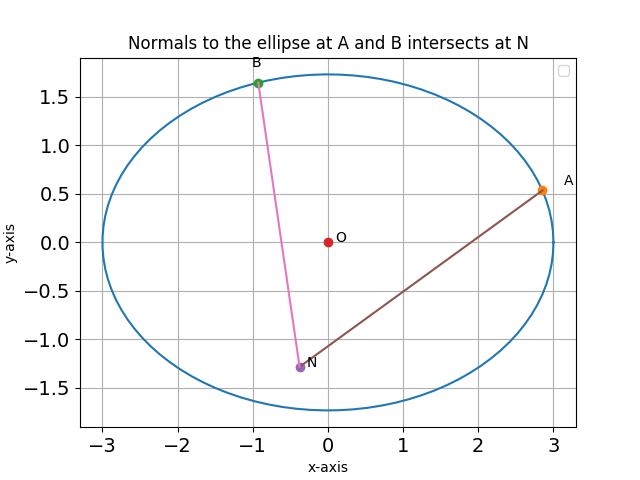
\includegraphics[scale=0.6]{preambule/Figure_2.png}

\end{frame}
\begin{frame}{Figure}
At $\theta =\frac{2\pi}{10}$
\centering
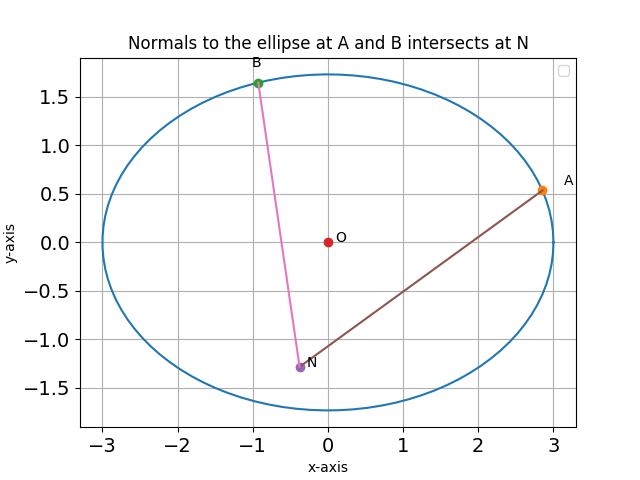
\includegraphics[scale=0.6]{preambule/Figure_3.png}
\end{frame}
\begin{frame}{Figure}
At $\theta =\frac{3\pi}{10}$
\centering
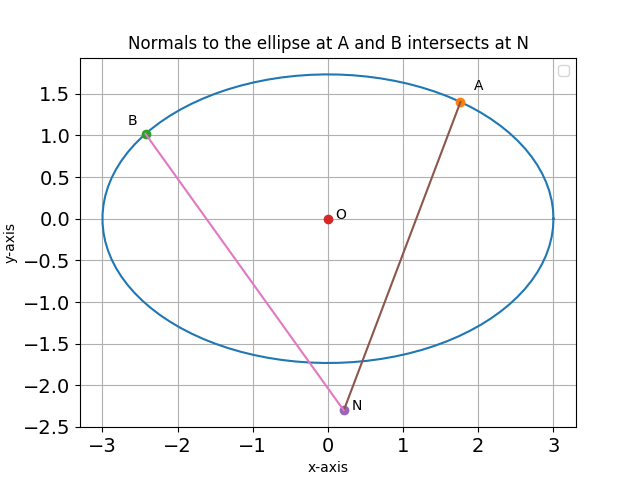
\includegraphics[scale=0.6]{preambule/Figure_4.png}

\end{frame}
\begin{frame}{Figure}
At $\theta =\frac{4\pi}{10}$
\centering
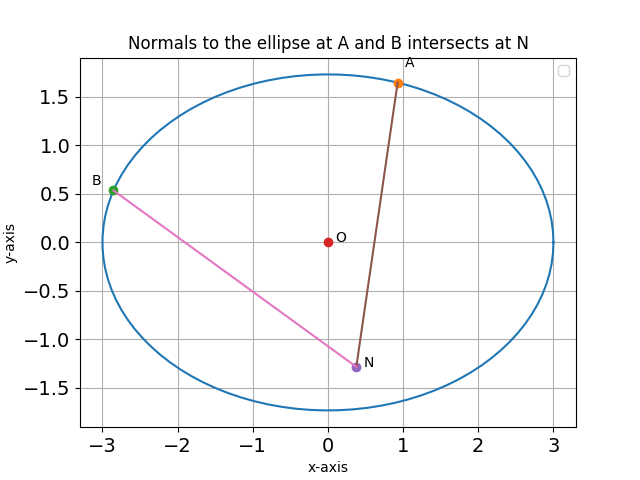
\includegraphics[scale=0.6]{preambule/Figure_5.png}

\end{frame}
\begin{frame}{Figure}

At $\theta =\frac{5\pi}{10}$
\centering
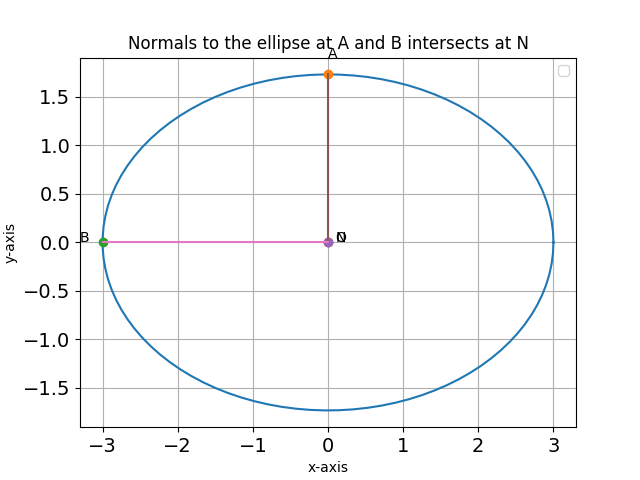
\includegraphics[scale=0.6]{preambule/Figure_6.png}

\end{frame}
\appendix\textbf{}
\section<presentation>*{\appendixname}
\subsection<presentation>*{Reference}

\begin{frame}[allowframebreaks]
  \frametitle<presentation>{References}
    
  \begin{thebibliography}{10}
 
  \beamertemplatearticlebibitems

  \bibitem{Sharma}
    G. V. V. ~Sharma.
    \newblock EE1390
    \newblock {\em Introduction to AI and ML}, Spring,
    2019.\\
    \url{github.com/gadepall/school/tree/master/linalg}
\beamertemplatearticlebibitems

  \bibitem{Online}
    Latex Beamer
    \url{https://www.overleaf.com/learn/latex/Beamer}
    
  \end{thebibliography}
\end{frame}

\end{document}
